
\documentclass[journal]{IEEEtran}

% Some very useful LaTeX packages include:
% (uncomment the ones you want to load)

% *** MISC UTILITY PACKAGES ***
%
%\usepackage{ifpdf}
% Heiko Oberdiek's ifpdf.sty is very useful if you need conditional
% compilation based on whether the output is pdf or dvi.
% usage:
% \ifpdf
%   % pdf code
% \else
%   % dvi code
% \fi
% The latest version of ifpdf.sty can be obtained from:
% http://www.ctan.org/tex-archive/macros/latex/contrib/oberdiek/
% Also, note that IEEEtran.cls V1.7 and later provides a builtin
% \ifCLASSINFOpdf conditional that works the same way.
% When switching from latex to pdflatex and vice-versa, the compiler may
% have to be run twice to clear warning/error messages.






% *** CITATION PACKAGES ***
%


% *** GRAPHICS RELATED PACKAGES ***
%
\ifCLASSINFOpdf
  % \usepackage[pdftex]{graphicx}
  % declare the path(s) where your graphic files are
  % \graphicspath{{../pdf/}{../jpeg/}}
  % and their extensions so you won't have to specify these with
  % every instance of \includegraphics
  % \DeclareGraphicsExtensions{.pdf,.jpeg,.png}
\else
  % or other class option (dvipsone, dvipdf, if not using dvips). graphicx
  % will default to the driver specified in the system graphics.cfg if no
  % driver is specified.
  % \usepackage[dvips]{graphicx}
  % declare the path(s) where your graphic files are
  % \graphicspath{{../eps/}}
  % and their extensions so you won't have to specify these with
  % every instance of \includegraphics
  % \DeclareGraphicsExtensions{.eps}
\fi
% graphicx was written by David Carlisle and Sebastian Rahtz. It is
% required if you want graphics, photos, etc. graphicx.sty is already
% installed on most LaTeX systems. The latest version and documentation can
% be obtained at: 
% http://www.ctan.org/tex-archive/macros/latex/required/graphics/
% Another good source of documentation is "Using Imported Graphics in
% LaTeX2e" by Keith Reckdahl which can be found as epslatex.ps or
% epslatex.pdf at: http://www.ctan.org/tex-archive/info/
%
% latex, and pdflatex in dvi mode, support graphics in encapsulated
% postscript (.eps) format. pdflatex in pdf mode supports graphics
% in .pdf, .jpeg, .png and .mps (metapost) formats. Users should ensure
% that all non-photo figures use a vector format (.eps, .pdf, .mps) and
% not a bitmapped formats (.jpeg, .png). IEEE frowns on bitmapped formats
% which can result in "jaggedy"/blurry rendering of lines and letters as
% well as large increases in file sizes.
%
% You can find documentation about the pdfTeX application at:
% http://www.tug.org/applications/pdftex





% *** MATH PACKAGES ***
%
\usepackage[cmex10]{amsmath}


% *** ALIGNMENT PACKAGES ***
%
\usepackage{array}
\usepackage{mdwmath}
\usepackage{mdwtab}
\usepackage{float}



% IEEEtran contains the IEEEeqnarray family of commands that can be used to
% generate multiline equations as well as matrices, tables, etc., of high
% quality.


%\usepackage{eqparbox}
% Also of notable interest is Scott Pakin's eqparbox package for creating
% (automatically sized) equal width boxes - aka "natural width parboxes".
% Available at:
% http://www.ctan.org/tex-archive/macros/latex/contrib/eqparbox/





% *** SUBFIGURE PACKAGES ***
%\usepackage[tight,footnotesize]{subfigure}
% subfigure.sty was written by Steven Douglas Cochran. This package makes it
% easy to put subfigures in your figures. e.g., "Figure 1a and 1b". For IEEE
% work, it is a good idea to load it with the tight package option to reduce
% the amount of white space around the subfigures. subfigure.sty is already
% installed on most LaTeX systems. The latest version and documentation can
% be obtained at:
% http://www.ctan.org/tex-archive/obsolete/macros/latex/contrib/subfigure/
% subfigure.sty has been superceeded by subfig.sty.


\usepackage[justification=centering]{caption}
%\usepackage[caption=false]{caption}
%\usepackage[font=footnotesize]{subfig}
% subfig.sty, also written by Steven Douglas Cochran, is the modern
% replacement for subfigure.sty. However, subfig.sty requires and
% automatically loads Axel Sommerfeldt's caption.sty which will override
% IEEEtran.cls handling of captions and this will result in nonIEEE style
% figure/table captions. To prevent this problem, be sure and preload
% caption.sty with its "caption=false" package option. This is will preserve
% IEEEtran.cls handing of captions. Version 1.3 (2005/06/28) and later 
% (recommended due to many improvements over 1.2) of subfig.sty supports
% the caption=false option directly:
%\usepackage[caption=false,font=footnotesize]{subfig}
%
% The latest version and documentation can be obtained at:
% http://www.ctan.org/tex-archive/macros/latex/contrib/subfig/
% The latest version and documentation of caption.sty can be obtained at:
% http://www.ctan.org/tex-archive/macros/latex/contrib/caption/




% *** FLOAT PACKAGES ***
%
%\usepackage{fixltx2e}
% fixltx2e, the successor to the earlier fix2col.sty, was written by
% Frank Mittelbach and David Carlisle. This package corrects a few problems
% in the LaTeX2e kernel, the most notable of which is that in current
% LaTeX2e releases, the ordering of single and double column floats is not
% guaranteed to be preserved. Thus, an unpatched LaTeX2e can allow a
% single column figure to be placed prior to an earlier double column
% figure. The latest version and documentation can be found at:
% http://www.ctan.org/tex-archive/macros/latex/base/



%\usepackage{stfloats}
% stfloats.sty was written by Sigitas Tolusis. This package gives LaTeX2e
% the ability to do double column floats at the bottom of the page as well
% as the top. (e.g., "\begin{figure*}[!b]" is not normally possible in
% LaTeX2e). It also provides a command:
%\fnbelowfloat
% to enable the placement of footnotes below bottom floats (the standard
% LaTeX2e kernel puts them above bottom floats). This is an invasive package
% which rewrites many portions of the LaTeX2e float routines. It may not work
% with other packages that modify the LaTeX2e float routines. The latest
% version and documentation can be obtained at:
% http://www.ctan.org/tex-archive/macros/latex/contrib/sttools/
% Documentation is contained in the stfloats.sty comments as well as in the
% presfull.pdf file. Do not use the stfloats baselinefloat ability as IEEE
% does not allow \baselineskip to stretch. Authors submitting work to the
% IEEE should note that IEEE rarely uses double column equations and
% that authors should try to avoid such use. Do not be tempted to use the
% cuted.sty or midfloat.sty packages (also by Sigitas Tolusis) as IEEE does
% not format its papers in such ways.


%\ifCLASSOPTIONcaptionsoff
%  \usepackage[nomarkers]{endfloat}
% \let\MYoriglatexcaption\caption
% \renewcommand{\caption}[2][\relax]{\MYoriglatexcaption[#2]{#2}}
%\fi
% endfloat.sty was written by James Darrell McCauley and Jeff Goldberg.
% This package may be useful when used in conjunction with IEEEtran.cls'
% captionsoff option. Some IEEE journals/societies require that submissions
% have lists of figures/tables at the end of the paper and that
% figures/tables without any captions are placed on a page by themselves at
% the end of the document. If needed, the draftcls IEEEtran class option or
% \CLASSINPUTbaselinestretch interface can be used to increase the line
% spacing as well. Be sure and use the nomarkers option of endfloat to
% prevent endfloat from "marking" where the figures would have been placed
% in the text. The two hack lines of code above are a slight modification of
% that suggested by in the endfloat docs (section 8.3.1) to ensure that
% the full captions always appear in the list of figures/tables - even if
% the user used the short optional argument of \caption[]{}.
% IEEE papers do not typically make use of \caption[]'s optional argument,
% so this should not be an issue. A similar trick can be used to disable
% captions of packages such as subfig.sty that lack options to turn off
% the subcaptions:
% For subfig.sty:
% \let\MYorigsubfloat\subfloat
% \renewcommand{\subfloat}[2][\relax]{\MYorigsubfloat[]{#2}}
% For subfigure.sty:
% \let\MYorigsubfigure\subfigure
% \renewcommand{\subfigure}[2][\relax]{\MYorigsubfigure[]{#2}}
% However, the above trick will not work if both optional arguments of
% the \subfloat/subfig command are used. Furthermore, there needs to be a
% description of each subfigure *somewhere* and endfloat does not add
% subfigure captions to its list of figures. Thus, the best approach is to
% avoid the use of subfigure captions (many IEEE journals avoid them anyway)
% and instead reference/explain all the subfigures within the main caption.
% The latest version of endfloat.sty and its documentation can obtained at:
% http://www.ctan.org/tex-archive/macros/latex/contrib/endfloat/
%
% The IEEEtran \ifCLASSOPTIONcaptionsoff conditional can also be used
% later in the document, say, to conditionally put the References on a 
% page by themselves.





% *** PDF, URL AND HYPERLINK PACKAGES ***
%
%\usepackage{url}
% url.sty was written by Donald Arseneau. It provides better support for
% handling and breaking URLs. url.sty is already installed on most LaTeX
% systems. The latest version can be obtained at:
% http://www.ctan.org/tex-archive/macros/latex/contrib/misc/
% Read the url.sty source comments for usage information. Basically,
% \url{my_url_here}.




\usepackage[backend=bibtex,style=ieee]{biblatex}
\addbibresource{IEEEabrv,report}

\usepackage{graphicx}
\usepackage{tikz}
\usetikzlibrary{arrows,positioning,shapes.geometric}


% *** Do not adjust lengths that control margins, column widths, etc. ***
% *** Do not use packages that alter fonts (such as pslatex).         ***
% There should be no need to do such things with IEEEtran.cls V1.6 and later.
% (Unless specifically asked to do so by the journal or conference you plan
% to submit to, of course. )


% correct bad hyphenation here
\hyphenation{op-tical net-works semi-conduc-tor}

\renewcommand{\arraystretch}{1.25}

\begin{document}
%
% paper title
% can use linebreaks \\ within to get better formatting as desired
\title{Condenser Microphone}
%
%
% author names and IEEE memberships
% note positions of commas and nonbreaking spaces ( ~ ) LaTeX will not break
% a structure at a ~ so this keeps an author's name from being broken across
% two lines.
% use \thanks{} to gain access to the first footnote area
% a separate \thanks must be used for each paragraph as LaTeX2e's \thanks
% was not built to handle multiple paragraphs
%

\author{A.~Sheikh,
				J.~Sakai,
				\IEEEmembership{Electrical~and~Computer~Engineering, Carnegie~Mellon}% <-this % stops a space
}

% The paper headers
\markboth{18-510 Capstone Design Report: 05/05/2014}{Sheikh, Sakai}

% The only time the second header will appear is for the odd numbered pages
% after the title page when using the twoside option.
% 
% *** Note that you probably will NOT want to include the author's ***
% *** name in the headers of peer review papers.                   ***
% You can use \ifCLASSOPTIONpeerreview for conditional compilation here if
% you desire.


% make the title area
\maketitle


\begin{abstract}
%\boldmath
For the application of accurate voice reproduction, a cost-effective condenser microphone design is considered. Analysis of theoretical characteristics such as sensitivity, dynamic range, and signal-to-noise ratio is presented. In conclusion, quantitative measurements from a working prototype are corroborated with the theoretical analysis.
\end{abstract}
% IEEEtran.cls defaults to using nonbold math in the Abstract.
% This preserves the distinction between vectors and scalars. However,
% if the journal you are submitting to favors bold math in the abstract,
% then you can use LaTeX's standard command \boldmath at the very start
% of the abstract to achieve this. Many IEEE journals frown on math
% in the abstract anyway.

% Note that keywords are not normally used for peerreview papers.
\begin{IEEEkeywords}
Capacitive, Condenser, Microphone.
\end{IEEEkeywords}

% For peer review papers, you can put extra information on the cover
% page as needed:
% \ifCLASSOPTIONpeerreview
% \begin{center} \bfseries EDICS Category: 3-BBND \end{center}
% \fi
%
% For peerreview papers, this IEEEtran command inserts a page break and
% creates the second title. It will be ignored for other modes.
\IEEEpeerreviewmaketitle



\section{Introduction}

\IEEEPARstart{T}{he} accurate transduction of sound into an electrical signal is naturally useful for conveying the human voice. People generally speak at 40~to~60~dB~SPL and can hear sound from 20~Hz~up~to~20~kHz with especial sensitivity to the 1~to~4~kHz region.\supercite{smith} For the application of accurate sound reproduction, the designer should strive for unity-gain response in these ranges, particularly in the 1~to~4~kHz range.

\begin{figure}[ht]
  \centering
	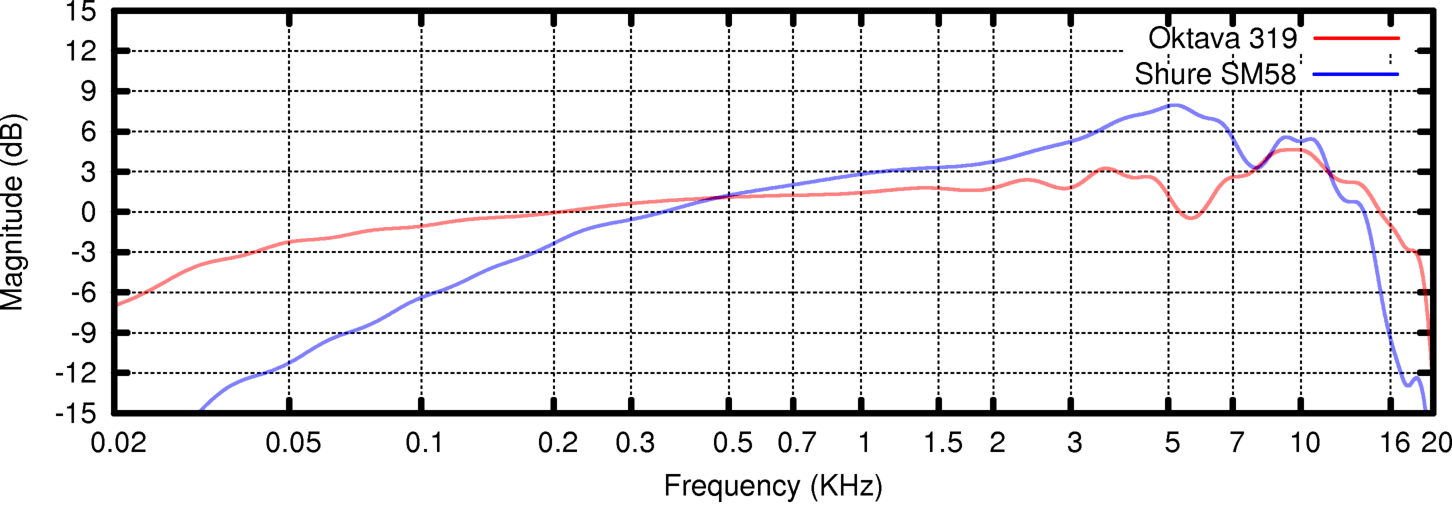
\includegraphics[width=0.45\textwidth]{OktavaMK319vsShureSM58.png}
  \caption{\em Oktava~MK-319 condenser microphone~\supercite{oktava} and Shure~SM58 dynamic microphone\supercite{shure} (20~Hz to 20~kHz)}
	\label{fig:OktavaMK319vsShureSM58}
\end{figure}

A variety of devices exist for transducing sound. Of commercially viable designs, condenser and dynamic microphones are the most common.~\supercite{shambro} Fig. \ref{fig:OktavaMK319vsShureSM58} plots the responses of a condenser microphone and a dynamic microphone. The condenser mic (in red) experiences less attenuation at the extremes and provides greater uniformity in between. It is not unusual for condenser mics to have an upper 20~kHz frequency limit compared to the typical 16~kHz limit experienced by dynamic mics.~\supercite{white} Additionally, the condenser microphone has notably less gain in the 1~to~4~kHz region people are most sensitive to, providing a more balanced response. Generalizing these results, condenser microphones are preferable for applications desiring accurate reproduction.

\begin{figure}[ht]
  \centering
	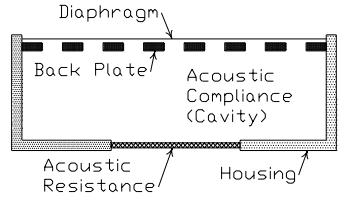
\includegraphics[scale=0.5]{DiaphragmSystem.png}
  \caption{\em Diaphragm system vertical cross-section~\supercite{torio}}
	\label{fig:DiaphragmSystem}
\end{figure}

\section{Sensor Structure and Measurement Principle}

\begin{figure}[ht]
	\centering
	\begin{tikzpicture}[auto, node distance=2cm,>=latex']
		\tikzstyle{round4} = [rectangle, draw, rounded corners, text centered, minimum height=2em, minimum width=10em, node distance=4.5cm]
		\tikzstyle{round1} = [rectangle, draw, rounded corners, text centered, minimum height=2em, minimum width=10em, node distance=1.25cm]
		\tikzstyle{header} = [draw=none, text centered, node distance=0.75cm]
		\tikzstyle{arrow} = [thick,->,>=stealth]
		
		\node (mechanical) [header, above of=sound] {\bf Mechanical};
		\node (electrical) [header, right of=mechanical, node distance=4.5cm] {\bf Electrical};
		\node (sound) [round1] {sound pressure};
		\node (gradient) [round1, below of=sound] {pressure gradient};
		\node (deflection) [round1, below of=gradient] {membrane deflection};
		\node (capacitance) [round4, right of=sound] {$\Delta$ capacitance};
		\node (voltage) [round4, right of=gradient] {$\Delta$ voltage};
		\node (preamp) [round4, right of=deflection] {preamplifier};
		
		\draw [arrow] (sound) -- (gradient);
		\draw [arrow] (gradient) -- (deflection);
		\draw [arrow] (deflection) -- (2.25,-2.5) -- (2.25,0) -- (capacitance);
		
		\draw [arrow] (capacitance) -- (voltage);
		\draw [arrow] (voltage) -- (preamp);
	\end{tikzpicture}
	\caption{\em Transducer signal chain, first the mechanical process, then the coupled electrical response}
	\label{fig:SignalChain}
\end{figure}

The diaphragm portion of the condenser microphone has a cylindrical form-factor. Its vertical cross-section is depicted in Fig. \ref{fig:DiaphragmSystem}. The diaphragm itself is a thin, tensioned membrane which is responsive to sound pressure in the target frequency range. The back-plate is a rigid structure with distributed holes leading to an internal cavity. Between the membrane and the back-plate is the air-gap which forms the condenser dielectric. An acoustic resistance at the rear of the internal cavity serves as a normalizing vent, allowing the cavity to equalize to atmospheric pressure.

Condenser microphones convert sound pressure into a voltage signal by the process shown in Fig. \ref{fig:SignalChain}. In the process, sound pressure gives rise to a pressure gradient which causes deflection across the condenser diaphragm. Membrane deflection in turn  causes the capacitance of the condenser to vary. Variations in capacitance produce corresponding changes in voltage on the biasing circuit the condenser is tied to. The resultant AC small-signal can then be extracted from the circuit and fed through a preamplifier to obtain a low output impedance voltage signal representing the source sound.

\begin{figure}[ht]
	\centering
	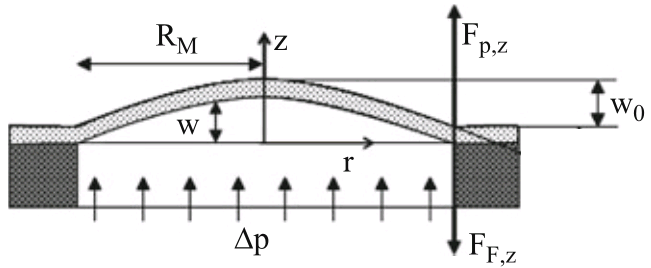
\includegraphics[scale=0.35]{MembraneDeflection.png}
	
	\begin{equation}
		\Delta p = \frac{4w_0 d_m}{R_M^2} \frac{E_M}{1-v_M^2} \left( \frac{4}{3} \frac{d_M^2}{R_M^2} + \sigma_0 + \frac{64}{105} \frac{w_0^2}{R_M^2} \right)
		\label{eq:Apex}
	\end{equation}
	
	\begin{equation}
		w(r) = w_0\left(1-\frac{r^2}{R_M^2}\right)
		\label{eq:Deflection}
	\end{equation}
	
	\begin{tabular}{ c | l }
		\hline
		\bf Symbol & \bf Description \\
		\hline
		$r$ & radius in cylindrical coordinates \\
		$R_M$ & membrane radius \\
		$d_M$ & membrane thickness \\
		$w$ & deflection along $z$-axis at a particular radius \\
		$w_0$ & apex of deflection, equal to $w(r=0)$ \\
		$P_0$ & atmospheric pressure \\
		$\Delta p$ & change in pressure relative to $P_0$ caused by sound \\
		$F_{p,z}$ & force due to uniform pressure across membrane \\
		$F_{f,z}$ & force due to membrane tension and frame \\
		$\sigma_0$ & residual stress, modeled with $\sigma_0=0$ \\
		$E_M$ & Young's Modulus of elasticity for the membrane \\
		$v_M$ & Poisson's ratio for the membrane \\
	\end{tabular}
	
	\caption{\em Modeled parabolic membrane deflection owing to uniform sound pressure\supercite{schomburg}}
	\label{fig:MembraneDeflection}
\end{figure}

\subsection{Membrane Deflection}

When sound pressure impinges upon the membrane, it oscillates with the pressure according to its mechanical properties. Fig. \ref{fig:MembraneDeflection} shows modeled parabolic deflection in cylindrical coordinates. The model assumes sound pressure is uniformly distributed across the face of the membrane. This produces purely vertical membrane oscillation along the $z$-axis in cylindrical coordinates, with the apex deflection $w_0$ occurring at the center of the membrane owing to the maximized moment arm at that point.

Setting residual stress $\sigma_0=0$, we can solve for the apex deflection using the relation shown in Eq. \ref{eq:Apex}\supercite{schomburg}. The apex deflection $w_0$ can then be used to calculate the modeled parabolic deflection at any radius $r$ with Eq. \ref{eq:Deflection}.

\subsection{Capacitance}

Let the back-plate be held at $z=h_0$ above the membrane to create the dielectric air-gap. Assume there is sound pressure and the membrane has a positive apex deflection $w_0>0$ and is deflected up towards the back-plate. If we treat the face of the membrane as a collection of cylindrical area differentials with $dA = r\,dr\,d\theta$ we can find the total capacitance under deflection by integrating the differential capacitances $dC$ as shown in Eq. \ref{eq:DifferentialCapacitance} and \ref{eq:DeflectedCapacitance}.

\begin{figure}[ht]
	\begin{equation}
		\int_A dC = \int_A \frac{\epsilon_0\,dA}{h_0-w(r)} %= \int_0^{R_M} \int_0^{2\pi} \frac{\epsilon_0 r}{h_0-w(r)}\,d\theta\,dr
		\label{eq:DifferentialCapacitance}
	\end{equation}
	
	\begin{equation}
		C = \frac{\pi\epsilon_0 R_M^2}{w_0} \mathrm{ln}\left(\frac{h_0}{h_0-w_0}\right)
		\label{eq:DeflectedCapacitance}
	\end{equation}
\end{figure}


%Negative apex deflection $w_0<0$ indicates deflection \emph{away} from the back-plate and produces the expression $h_0+|w_0|$ in the denominator of the natural logarithm.

\subsection{Voltage}


% An example of a floating figure using the graphicx package.
% Note that \label must occur AFTER (or within) \caption.
% For figures, \caption should occur after the \includegraphics.
% Note that IEEEtran v1.7 and later has special internal code that
% is designed to preserve the operation of \label within \caption
% even when the captionsoff option is in effect. However, because
% of issues like this, it may be the safest practice to put all your
% \label just after \caption rather than within \caption{}.
%
% Reminder: the "draftcls" or "draftclsnofoot", not "draft", class
% option should be used if it is desired that the figures are to be
% displayed while in draft mode.
%
%\begin{figure}[!t]
%\centering
%\includegraphics[width=2.5in]{myfigure}
% where an .eps filename suffix will be assumed under latex, 
% and a .pdf suffix will be assumed for pdflatex; or what has been declared
% via \DeclareGraphicsExtensions.
%\caption{Simulation Results}
%\label{fig_sim}
%\end{figure}

% Note that IEEE typically puts floats only at the top, even when this
% results in a large percentage of a column being occupied by floats.


% An example of a double column floating figure using two subfigures.
% (The subfig.sty package must be loaded for this to work.)
% The subfigure \label commands are set within each subfloat command, the
% \label for the overall figure must come after \caption.
% \hfil must be used as a separator to get equal spacing.
% The subfigure.sty package works much the same way, except \subfigure is
% used instead of \subfloat.
%
%\begin{figure*}[!t]
%\centerline{\subfloat[Case I]\includegraphics[width=2.5in]{subfigcase1}%
%\label{fig_first_case}}
%\hfil
%\subfloat[Case II]{\includegraphics[width=2.5in]{subfigcase2}%
%\label{fig_second_case}}}
%\caption{Simulation results}
%\label{fig_sim}
%\end{figure*}
%
% Note that often IEEE papers with subfigures do not employ subfigure
% captions (using the optional argument to \subfloat), but instead will
% reference/describe all of them (a), (b), etc., within the main caption.


% An example of a floating table. Note that, for IEEE style tables, the 
% \caption command should come BEFORE the table. Table text will default to
% \footnotesize as IEEE normally uses this smaller font for tables.
% The \label must come after \caption as always.
%
%\begin{table}[!t]
%% increase table row spacing, adjust to taste
%\renewcommand{\arraystretch}{1.3}
% if using array.sty, it might be a good idea to tweak the value of
% \extrarowheight as needed to properly center the text within the cells
%\caption{An Example of a Table}
%\label{table_example}
%\centering
%% Some packages, such as MDW tools, offer better commands for making tables
%% than the plain LaTeX2e tabular which is used here.
%\begin{tabular}{|c||c|}
%\hline
%One & Two\\
%\hline
%Three & Four\\
%\hline
%\end{tabular}
%\end{table}


% Note that IEEE does not put floats in the very first column - or typically
% anywhere on the first page for that matter. Also, in-text middle ("here")
% positioning is not used. Most IEEE journals use top floats exclusively.
% Note that, LaTeX2e, unlike IEEE journals, places footnotes above bottom
% floats. This can be corrected via the \fnbelowfloat command of the
% stfloats package.



\section{Conclusion}
The conclusion goes here.





% if have a single appendix:
%\appendix[Proof of the Zonklar Equations]
% or
%\appendix  % for no appendix heading
% do not use \section anymore after \appendix, only \section*
% is possibly needed

% use appendices with more than one appendix
% then use \section to start each appendix
% you must declare a \section before using any
% \subsection or using \label (\appendices by itself
% starts a section numbered zero.)
%


%\appendices
%\section{Proof of the First Zonklar Equation}
%Appendix one text goes here.

% you can choose not to have a title for an appendix
% if you want by leaving the argument blank
%\section{}
%Appendix two text goes here.


% use section* for acknowledgement
%\section*{Acknowledgment}


%The authors would like to thank...


% Can use something like this to put references on a page
% by themselves when using endfloat and the captionsoff option.
\ifCLASSOPTIONcaptionsoff
  \newpage
\fi



% trigger a \newpage just before the given reference
% number - used to balance the columns on the last page
% adjust value as needed - may need to be readjusted if
% the document is modified later
%\IEEEtriggeratref{8}
% The "triggered" command can be changed if desired:
%\IEEEtriggercmd{\enlargethispage{-5in}}

% references section

% can use a bibliography generated by BibTeX as a .bbl file
% BibTeX documentation can be easily obtained at:
% http://www.ctan.org/tex-archive/biblio/bibtex/contrib/doc/
% The IEEEtran BibTeX style support page is at:
% http://www.michaelshell.org/tex/ieeetran/bibtex/
%\bibliographystyle{IEEEtran}
% argument is your BibTeX string definitions and bibliography database(s)
%\bibliography{IEEEabrv,../bib/paper}
%
% <OR> manually copy in the resultant .bbl file
% set second argument of \begin to the number of references
% (used to reserve space for the reference number labels box)
%\begin{thebibliography}{1}

%\bibitem{IEEEhowto:kopka}
%H.~Kopka and P.~W. Daly, \emph{A Guide to \LaTeX}, 3rd~ed.\hskip 1em plus
%  0.5em minus 0.4em\relax Harlow, England: Addison-Wesley, 1999.

%\end{thebibliography}

% You can push biographies down or up by placing
% a \vfill before or after them. The appropriate
% use of \vfill depends on what kind of text is
% on the last page and whether or not the columns
% are being equalized.

%\vfill

% Can be used to pull up biographies so that the bottom of the last one
% is flush with the other column.
%\enlargethispage{-5in}

\printbibliography

% that's all folks
\end{document}


